\documentclass[main.tex]{subfiles}

\graphicspath{{./img}}
\begin{document}
\section{Intelligent Transport Systems}\label{its}

Intelligent transport systems describe an initiative to utilize modern technology 
to optimize and increase efficiency of processes common to the domain of transportation. 
This usually involves enabling different actors in the transportation system to communicate 
with each other and share available information (much like multi-agent systems). With the 
availability of shared information, complex, data-driven systems can be built utilizing 
state-of-the-art tech concepts like machine learning, computer vision and IoT while
integrating humans, roads and automobiles, improved street protection, efficiency and stability.
İt also address environmental issues via controlling traffic to prevent congestions or lessen
their adverse effects.

\begin{figure}[htbp]
    \centering
    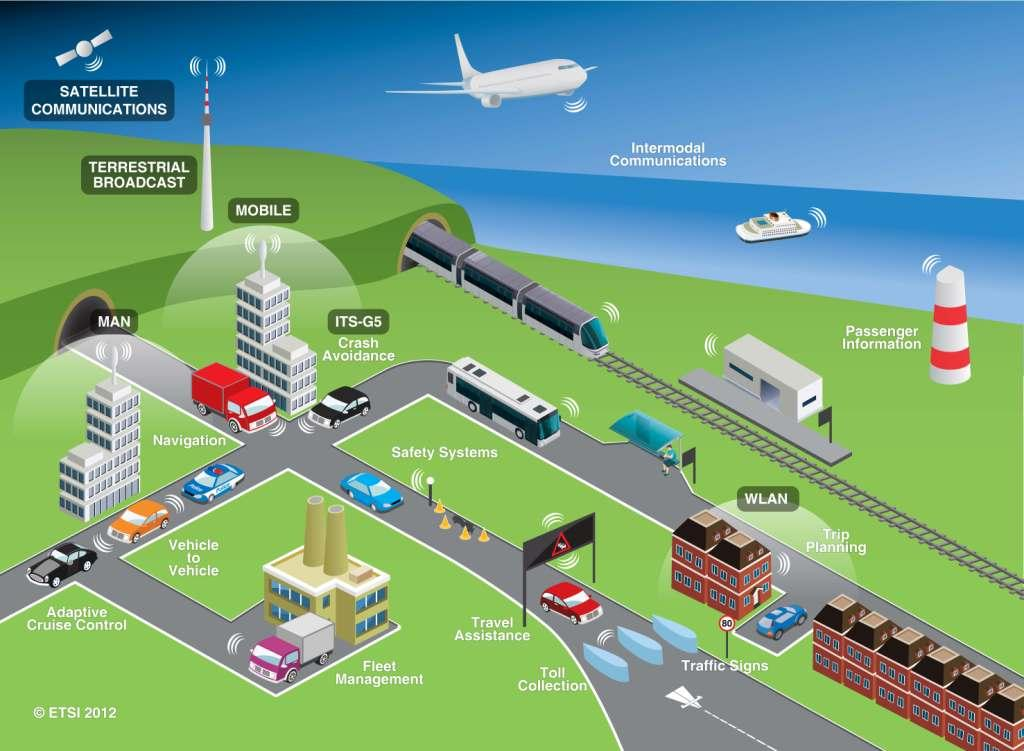
\includegraphics[width=.8\textwidth]{ITS-schema.jpg}
    \caption{Illustration of an ITS topology \cite{ETSI}}
    \label{its-map}
\end{figure}

ITS can provide itself most useful in the following aspects of transportation: 
\emph{Mobility}, \emph{Safety}, \emph{Environment}. To provide an example, regarding mobility, 
one of the most common system is routing and navigation for road vehicles. Such systems can 
factor in time, distance and even emissions when providing route guidance. This leads to 
increased performance of road networks. Regarding safety, one can mention emergency management
systems like E-Call, which provides automated post-crash assistance by contacting emergency
services as soon as an incident happens. In terms of the environment, 
ITS allows for demand management through \emph{electronic fee collection}, which allows for 
flexible charges for road usage, based on vehicle type and emissions category. \cite{Commision2022}
Another, more general example of emissions reduction of ITS is through reducing congestions, as road vehicle 
emissions have proven to be a significant environmental factor not only in emission production
per se, but also one that humans are most exposed to. In a study conducted by the Harvard
School of Public Health, air pollution from traffic congestion in 83 of the USA's largest urban
areas contributes to more than 2,200 premature deaths annually, costing the health system at
least \$18 billion \cite{Levy2011}.

\subsection{Implementation}

In relation to the topic of this thesis, it is important to define ITS features that will create a
qualitative analysis/benchmark for identifying suitable system(s) for the ITS implementation. The following 
sections will discuss and features that will be used for reasoning which ITS to implement in the 
practical part of this thesis.

\subsubsection{Driver engagement}

Firstly, it is important to say that ITSs vary in terms of \emph{driver engagement}. Because
IVS's focus is to mainly research driver behaviour, a trivial requirement is to integrate with 
automotive transport. Furthermore, a system with a large degree of driver interaction should be
chosen to have an observable effect. 

As per (\ref{whyITS}), the ITS to develop/implement as part of the thesis having one or more of 
the following features should ensure high driver (i.e. user) engagement:

\begin{itemize}
    \itemspacing{.7}
    \item Geo-info service
    \item Real-time road condition service 
    \item Accurate traffic-info service 
    \item Real-time vehicle info service 
    \item Parking guidance service
\end{itemize}

\begin{figure}[htbp]
    \centering
    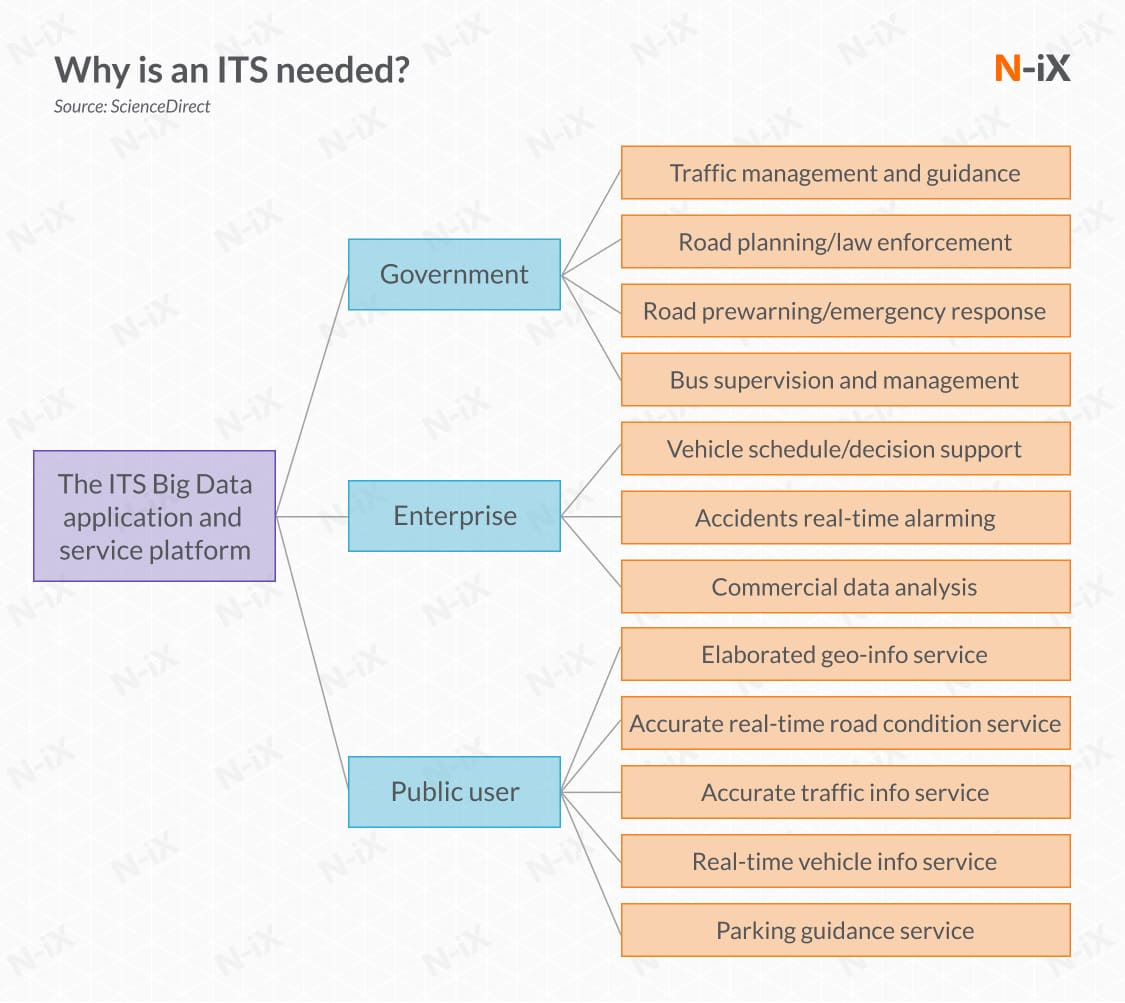
\includegraphics[width=.8\textwidth]{why is ITS needed.jpg}
    \caption{Reasons for ITS usage}
    \label{whyITS}
\end{figure}

\subsubsection{MAS-compatibility} \label{mas-compatibility}

Secondly, it is important to acknowledge whether there is an ITS that could be simulated using the MAS theory,
so that the information gathered in the first section of this thesis could be successfully applied.

Intelligent transport systems are, by nature, systems combining several actors together to achieve a common goal. 
Would this mean that every ITS can be, in fact, modelled as multi-agent system? The answer is
that it does \emph{not} apply for every one of them. 

Historically speaking, ITS that were
developed and proved helpful for optimizing traffic were \emph{centralized}, meaning there is a
single core in charge of logic and decision-making, organizing other units/actors within the
system, while interacting with the drivers in the traffic as external actors. The main
advantage of these systems is that they are less complex, therefore easier to develop a resilient,
safe product. The main drawback of this method is that they are heavily affected by the size
of instances, increasing the complexity and often result in exceedingly large computation time,
making the solution sub-optimal \cite{Corman2010}. 

As with the \emph{distributed} systems, the main challenge making individual agents 
solving sub-problem, cooperating well to achieve good and predictable results, as has been 
illustrated in section (\ref{mas}). Distributed systems can be used to solve traffic optimization
problems on a larger scale problems. These systems have seen larger usage especially in the
recent times, as newly produced vehicles are equipped with powerful computers that can be used
to transfer the computational burden from the core computer in centralized systems. Also
state-of-art communication protocols like DSRC and ITS 5G, which enable low-latency direct
communication between vehicles. 

The one example of an ITS where implementations have been carried out in both centralized and 
decentralized principles numerous times is a \emph{Network traffic control}. The goal of this 
system is to use knowledge about the traffic on the network to control traffic lights and other 
active traffic control elements to optimize traffic flow and decrease travel time. In \cite{Chow2019}, 
a centralized and distributed network traffic control systems were compared. The conclusion was that 
although the centralized system was able to achieve better performance higher global efficiency, 
the decentralized solution required significantly less computation time (40 \% in their experiment case).

Other decentralized, MAS-based systems that are more exposed to the user (driver) include the 
\emph{Adaptive Cruise Control} (ACC), for example. ACC extends the usual cruise control systems 
that maintain vehicle speed by adapting to speed of the vehicle upfront, if there is any. In fact, 
recent development has lead to a further improvement, making ACC a cooperative system (CACC) that 
enables vehicles to adopt a \emph{driving strategy} by communicating with the infrastructure (V2I 
communication).

\subsubsection{Current research}

Secondly, it is important to choose a system that is time-relevant and would bring benefit to
current as well as future IVS and HMI research activities. Therefore, the third quality for choosing 
an ITS to implement would be one that is still subject to research and current trends in 
the ITS industry and explore state-of-the-art ITS. In order to determine which ITSs are relevant, 
it is important to review ongoing project of governmental bodies and their strategies and also
current trends in automotive ITS research activities.

In Europe, there are initiatives to centralize decision making and ITS deployment on the scale of 
the European continent. The reason behind this initiative is quite clear - to enable Europe-wide 
interoperability between deployed ITS and ITS-enabled vehicles. It is without a question that 
such organization would closely work with the industry, helping to create conditions for novel 
ITS technologies to be deployed.

\paragraph{ERTICO}

One such European organization is \emph{ERTICO} (European Road Transport Telematics
Implementation Coordination - a public-private partnership organization
with close to 120~members, connecting 8 different sectors in the ITS Community, including
service providers, suppliers, traffic and transport industry, research institutions and
universities, public authorities, user organizations, connectivity industry as well as
vehicle manufacturers \cite{ertico}.

As of now, ERTICO's activities focus on the following areas:

\term{Connected Cooperative \& Automated Mobility}
As the computational power of newly-produced vehicles is increasing dramatically with every 
new generation, as well as the number of sensor data, ERTICO states their focus is on utilizing 
the large amounts of real-life data to deepen the machine learning models, as well as building 
an infrastructure that will allow handling this data. C-ITS (Cooperative Intelligent Transport
Systems) is also mentioned, whose principles are being put into practice by several projects, 
namely European Truck Platooning (ETPC), ADASIS (Advanced map-enhanced driver assistance systems) and 
more. ERTICO's main contribution is to facilitate creation of ITS ecosystem by following a
multidisciplinary approach involving all relevant transport stakeholder sectors.

\term{Clean \& Eco- Mobility}
As has been already mentioned, smart mobility innovations make a major contribution towards 
reducing the impact of transport on emissions, which has got a non-negligible contribution to 
global greenhouse gas emissions production \cite{Ritchie2020}. Below are the four main
objectives in the are of Clean \& Eco-Mobility. 

\begin{itemize}
    \setlength\itemsep{-10pt}
    \item Develop a common approach to the evaluation of ITS deployment as a tool for emissions reduction
    \item Contribute to smart mobility solutions being recognized as a tool for reducing emissions
    \item Achieve interoperability of electro-mobility
    \item Contribute to creating an ICT network with seamless and interoperable electro-mobility services
\end{itemize}

\term{Urban Mobility}
Another focus of ERTICO is Urban Mobility, where the main goal is to provide "Mobility as a Service" (MaaS), 
which is a system that could decrease congestions and provide low-carbon and -emission multi-modal transport 
solutions.  

\term{Transport \& Logistics}
ERTICO states that the current European world of transport and logistics is too fragmented, so an effort to 
develop solution for connecting logistics information system would optimize cargo flows and facilitate supply 
chain management. 

In conclusion, the ERTICO organization helps to reduce time to market of innovative,
state-of-the-art technologies, increasing inter-operability between individual ITS by promoting
an open framework for integration and deployment of intelligent transport services. 

As described above, there are potential systems that are yet to be fully implemented and
deployed for consumer use. 

\paragraph{Cooperative ITS}

Cooperative Intelligent Transport Systems (C-ITS) refers to transport systems, where the
cooperation between two or more ITS sub-systems (personal, vehicle, roadside and central)
enables and provides an ITS service that offers better quality and an enhanced service level,
compared to the same ITS service provided by only one of the ITS sub-systems.\cite{2022} 
An example of the concept of the technology can be seen on the figure (\ref{c-its}) below. 

\begin{figure}[htbp]
    \centering
    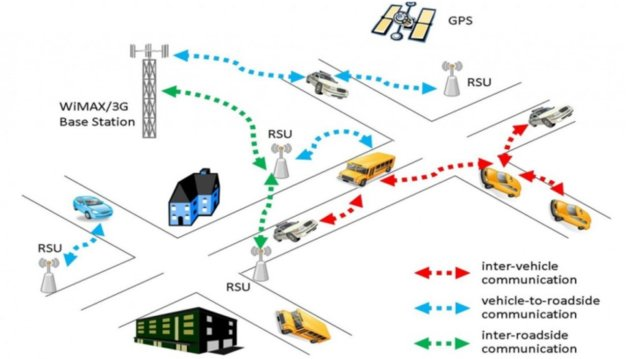
\includegraphics[width=.8\textwidth]{c-its.jpg}
    \caption{Example schematic of C-ITS scenario}
    \label{c-its}
\end{figure}

The concept of C-ITS was developed by the European Commission, representatives of industry and 
authorities in the European Union. In 2016, it was agreed on a coordinated establishment of intelligent
transport systems in Europe. It is considered to be one of the various tools to facilitate achieving 
the \emph{vision zero}, which is a project that aims to mitigate all fatalities involving road 
transport.

The European Commission outlined its plan for the coordinated deployment of C-ITS in Europe in
its communication 'A European strategy on Cooperative Intelligent Transport Systems', in which
it also states that the full-scale deployment of C-ITS services and C-ITS enabled vehicles is
expected to start in 2019.

The main feature of C-ITS is an intelligence that is distributed between vehicles and the infrastructure, 
which is a novel concept in the ITS world. Consequently, it is easy to see similarities to how 
MAS are described. Regarding the topic of this thesis, this could pose as an argument to
implement one of C-ITS systems in the practical part of this thesis, considering that  

Vehicles and infrastructure equipped with C-ITS can, for example, communicate a warning to each
other, after which the drivers are informed about the upcoming traffic situation in time for
them to take the necessary actions in order to avoid potential harm. Other potential benefits
of the use of C-ITS include reduced congestion and improved driver comfort. In short, vehicles 
share data directly between each other (V2V) and with the infrastructure (V2I) using ad-hoc
short range telecommunication. The two types of communications are sometimes together referred 
to as Vehicle-to-everything (V2X) communication.

This technology aims to benefit to both manually-driven vehicles 
as well as autonomous self-driving vehicles. The main use-cases, which were developed as
standalone services using C-ITS technology can be seen in the figure (\ref{c-its-use-case})
below.

\begin{figure}[htbp]
    \centering
    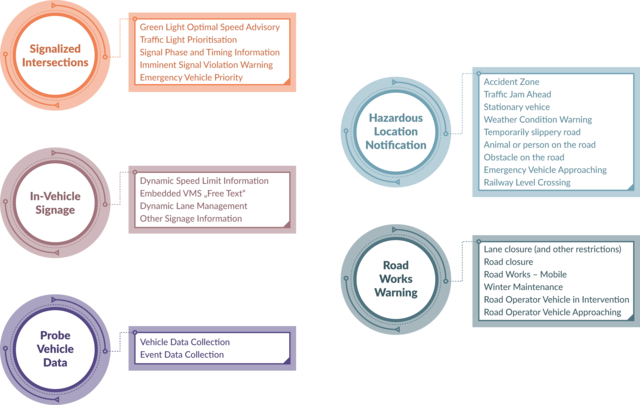
\includegraphics[width=.8\textwidth]{c-its-kolecka.png}
    \caption{C-ITS use cases \cite{2022}}
    \label{c-its-use-case}
\end{figure}

In general, the traffic safety and traffic flow improvements can be grouped based on which 
operational tasks they serve \cite{CRoads2021}: 

\begin{itemize}
    \item Provide \emph{information} to road users to improve road safety and comfort.
    \item Display \emph{regulatory boundaries} to inform road users of specific obligations, 
    restrictions or prohiitions
    \item Provide \emph{warnings} to road users about incidents ahead in their exact nature. 
\end{itemize}

\subparagraph{Project C-Roads}

In order to study the effects and refine the future deployment process of C-ITS, a project 
organized by the EU member states and road operators, called \emph{C-Roads} was established. 
The project's main objective is to harmonize C-ITS deployment activities across Europe. 
Within the C-Roads project, there have been established 5 work groups (WG), each focusing on a 
specific topic/scope regarding C-ITS objectives and priorities for research, testing and pre-
deployment of C-ITS \cite{Commision2021}. 

\begin{itemize}
    \itemspacing{0.7}
    \item WG1: Develop an EU agenda for testing
    \item WG2: Coordination and cooperation of R\&I activities
    \item WG3: Physical and digital road infrastructure
    \item WG4: Road Safety
    \item WG5: Access and exchange of data \& cyber-security
    \item WG6: Connectivity and digital infrastructure
\end{itemize}

Regarding the scope of this thesis, \emph{WG3} is the most informative segment. The focus of this group 
was in the first place regarding the infrastructure support for automated vehicles (SAE L4). One of 
the objectives was linking relevant physical and digital infrastructure, assessing relevance between 
them and automated vehicles, and mapping infrastructure elements to use-cases as \emph{generic driving 
tasks} (GDT):

\begin{itemize}
    \item Sensing \& Perception
    \begin{itemize}
        \itemspacing{.7}
        \item Ego localization
        \item Environmental awareness (object classification and incident detection)
        \item Enhanced perception (for limited visibility scenarios)
    \end{itemize}
    \item Planning
    \begin{itemize}
        \itemspacing{.7}
        \item (dynamic) information and regulations
        \item Safe and appropriate navigation plans
        \item Cooperative planning
    \end{itemize}
    \item Actuation
    \begin{itemize}
        \itemspacing{.7}
        \item Motion Control
        \item Minimum Risk Menoeuvre
    \end{itemize}
\end{itemize}

It is therefore advisable to keep these GDT in mind when choosing which ITS to develop 
regarding the thesis, because previous R\&I activities have shown that the tasks above will be a fundamental part 
of the future C-ITS deployment. Because all of the GDT seem to be more or less distinct
activities, the table below (\ref{gdt-mapping}) was created to map each GDT to particular C-ITS system, which
will be used to narrow down the potential ITS implementation candidates and hopefully make the final
decision for ITS implementation clear. 

\begin{table}[htbp]
    \caption{GDT to ITS mapping}
    \renewcommand{\arraystretch}{1.3}
    \centering\begin{tabular}{lp{7em}lp{10em}} \toprule
        \multicolumn{2}{c}{GDT} & \multicolumn{2}{c}{Mapping}                                                   \\ \cmidrule(r){1-2} \cmidrule(l){3-4}
        Group                   & Name                        & Type       & Description                        \\ \midrule
        \multirow{1}{3cm}
        {Sensing \& Perception} & Ego-localization            & HD Maps    & Geo-fencing                        \\
                                &                             & AD         & Self-driving algorithms            \\
                                & Environmental awareness     & IVIS       & Intersection Collision war.        \\
                                &                             &            & Emergency Vehicle war.             \\
                                &                             &            & Stationary Vehicle war.            \\
                                &                             &            & Traffic Jam war.                   \\
                                &                             &            & Traffic accident war.              \\
                                & Enhanced\newline perception & IVIS       & Overtaking war.                    \\
                                &                             &            & Intersection Collision war.        \\
                                &                             &            & VRU warning                        \\ \midrule
        Planning                & Information and regulations & CACC       & Green Light Optimal Speed Advisory \\
                                & Safe navigation plans       & Navigation & Dynamic Vehicle Routing            \\
                                & Cooperative planning        & AD         & Platooning                         \\ \midrule
        Actuation               & Motion Control              & AD         & Self-driving algorithms            \\
                                & Minimum Risk Menoeuvre      & AD         & Self-driving algorithms            \\ \midrule[1.0pt]
&&&\\
        \textbf{Legend}         &                             &            &                                    \\ \midrule
        Abbreviation            & Meaning                     &            &                                    \\ \midrule% \cmidrule(r){1-2}
        HD                      & \multicolumn{3}{l}
        {High-definition}                                                                                       \\
        AD                      & \multicolumn{3}{l}
        {Autonomous driving}                                                                                    \\
        IVIS                    & \multicolumn{3}{l}
        {In-Vehicle Information Systems}                                                                        \\
        VRU                     & \multicolumn{3}{l}
        {Vurneable Road User}                                                                                   \\
        CACC                    & \multicolumn{3}{l}
        {Cooperative Adaptive Cruise Control}                                                                   \\ \bottomrule
    \end{tabular}
    \label{gdt-mapping}
\end{table}
\clearpage
% \begin{table}[htbp]
%     \centering\begin{tabular}{ll} %\toprule
%         Abbreviation & Meaning                             \\ \midrule
%         HD           & High-definition                     \\
%         AD           & Autonomous driving                  \\
%         IVIS         & In-Vehicle Information Systems      \\
%         VRU          & Vurneable Road User                 \\
%         CACC         & Cooperative Adaptive Cruise Control \\ %\bottomrule
%     \end{tabular}
%     \caption{Legend for table \ref{gdt-mapping}}
%     \label{gdt-legend}
% \end{table}

\subsection{Qualitative analysis}

Looking at the table (\ref{gdt-mapping}), it is evident that all the tasks fall under \emph{four} 
mapping types. Those will be used as entries in the qualitative analysis. Nevertheless,
all types of ITS considered in the preceding sections will be examined and subsequently
evaluated to decide which type of ITS would be the most optimal to implement. 

The method to determine how well-suited the candidate system type is for the implementation to an IVS 
will be to evaluate it based on the \emph{three} features discussed in the preceding sections: 

\begin{itemize}
    \itemspacing{.5}
    \item MAS-compatibility
    \item Driver engagement
    \item Research relevance
\end{itemize}

A set of integer values will determine significance of each of the features. The significance
will be given in four levels:

\begin{itemize}
    \itemspacing{.5}
    \item \talign{None}{5}{$\rightarrow$\quad 0}
    \item \talign{Low}{5}{$\rightarrow$\quad 2}
    \item \talign{Moderate}{5}{$\rightarrow$\quad 5}
    \item \talign{High}{5}{$\rightarrow$\quad 8}
\end{itemize}

\begin{table}[htbp]
    \caption{Quantitative analysis results}
    \renewcommand{\arraystretch}{1.4}
    \centering\begin{tabular}{l*{3}{r}r} \toprule
         & \multicolumn{3}{c}{Features} & \\ \cmidrule(rl){2-4}
        ITS & \multicolumn{1}{p{6em}}{MAS-compatibility} & \multicolumn{1}{p{6em}}{Driver \newline engagement} & \multicolumn{1}{p{6em}}{Research \newline relevance} & Score \\ \midrule
        E-Call & 2 & 2 & 5 & 9 \\ 
        Electronic fee collection & 2 & 0 & 2 & 4 \\
        Parking guidance & 2 & 8 & 5 & 15 \\
        Network traffic control & 8 & 0 & 8 & 16 \\
        \textbf{Cooperative ACC} & 8 & 8 & 8 & \textbf{24} \\
        European Truck Platooning & 5 & 2 & 8 & 15 \\
        ADASIS & 2 & 8 & 8 & 18 \\
        Mobility as a Service & 8 & 2 & 8 & 18 \\
        Map services (Geo-fencing) & 2 & 5 & 8 & 15 \\
        \multicolumn{1}{p{5em}}{Self-driving algorithms} \& Platooning & 8 & 2 & 8 & 18 \\
        \textbf{IVIS} & 8 & 8 & 8 & \textbf{24} \\ \bottomrule
    \end{tabular}
    \label{qa-table}
\end{table}
\clearpage 

\subsection{In-Vehicle Information System}

The In-Vehicle Information System, shortly IVIS, is a term that comprises a vast number of vehicle technology 
solutions that assist the driver either by providing information about the vehicle and the surrounding environment 
or serving as an interface to control vehicle systems. 

The integral part is the \emph{Infotainment system} (fig. \ref{ivis-interface}), which is a
video/audio interface, providing control through elements such as touch screen button panel or
voice commands.  Moreover, it integrates other vehicle technology elements, such as the CAN
interface, connectivity modules (e.g. Wi-Fi, GPS), sensors etc \cite{Saxena}. A screen panel is
an excellent medium to provide additional safety information to the driver, especially when the
gauge clusters have been replaced by an additional screen which improves the HMI aspect by
reducing the disruptive effect of checking the screen and making the displayed information more
noticeable. 

The conventional, more basic capabilities of IVIS are HVAC control, multimedia controls, navigation support and 
parking assistance (i.e. parking camera view). These systems on their own, however, aren't valuable with regard 
to the thesis topic. The important feature of IVIS is the integration with the emerging C-ITS technologies, which 
greatly extend the capabilities of IVIS, i.e. displaying warning and awareness messages from the V2X interface. 
This fact makes IVIS a good candidate to implement to the IVS in the practical part, because the V2X C-ITS are 
a great subject for research as of now and the distributed nature of the systems corresponds to the agent-based 
requirement of the thesis topic. On top of that, the important HMI aspect of IVIS could provide great value for 
future utilization in research using IVS. 

The general idea for method of implementation is to implement C-ITS awareness and warning information system by 
simulating message-based communication between road users \& infrastructure and provide interface to display the 
information on the infotainment screen.

\begin{figure}[htbp]
    \centering
    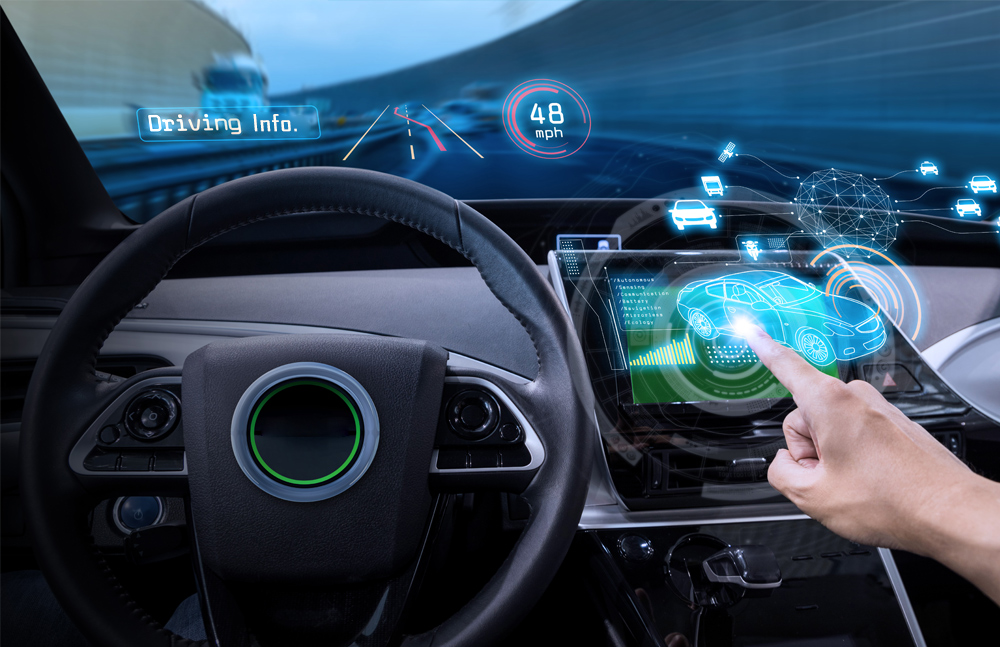
\includegraphics[width=.8\textwidth]{ivis-dashboard.jpg}
    \caption{Illustrative example of IVIS interface \cite{Saxena}}
    \label{ivis-interface}
\end{figure}

\subsection{Cooperative Adaptive Cruise Control}

The Cooperative Adapive Cruise Control (CACC) is an extension to an already well proven ITS - Adaptive Cruise Control.
As has been described above, this system extends the base cruise control by utilizing the V2V information broadcasted 
by other road users. The system has proved to reduce the number of shockwaves by reducing
oscillations that would otherwise happen without speed information sharing and increasing
capacity of the traffic network, albeit only with higher penetration rates ($\ge 40\%$)
\cite{van_Arem_2006}. Though, regarding the introduced thesis topic requirements, 
the system in itself doesn't provide any extra engagement from the driver side. 

However, another system that built upon the concept of CACC by utilizing information from the
infrastructure, namely the traffic signals, has been also recently developed this system can be
extended by information fs about signal phasing and consequently adopting a speed that would
eliminate the need to stop before a red light, avoiding idle time. The system is called
\emph{Green Light Optimization Speed Advisory} (GLOSA). According to \cite{Pariota_2019}, the results 
of simulating deployment of this system demonstrated that even using a simple
control algorithm with the aim to avoid the stop\&go a reduction of fuel consumption
and emissions in the region of 5 to 12 \% has been observed. The study in \cite{Katsaros_2011} even 
concluded that with enough penetration, the idle (stop) time could be decreased by more than $70 \%$ 
(see fig. \ref{glosa-chart} below).

The the proposed idea for simulating the system in an IVS would be to implement a GLOSA traffic controller 
algorithm and use the C-ITS information system to provide the driver with the optimal speed information, which 
would be displayed on the infotainment screen.

\begin{figure}[htbp]
    \centering
    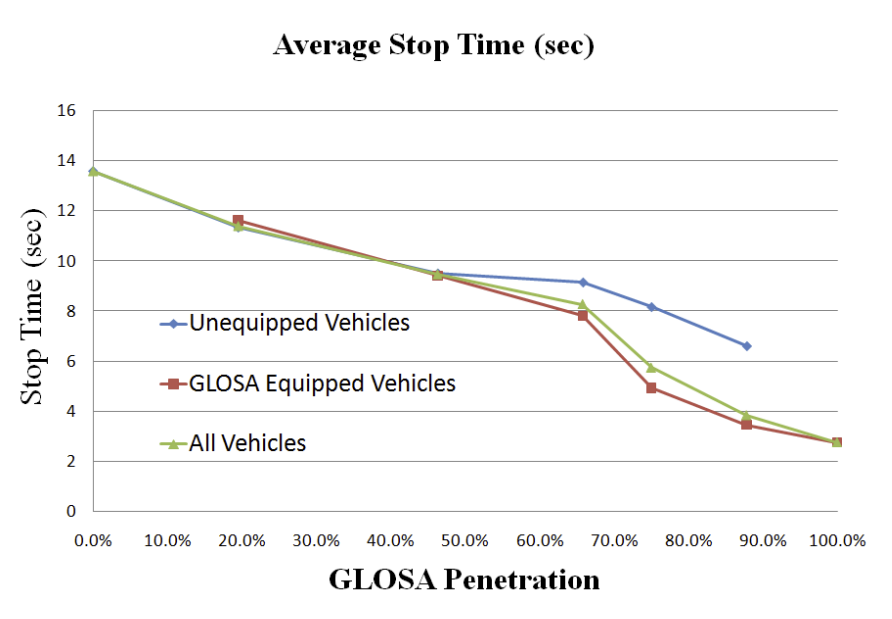
\includegraphics[width=.8\textwidth]{glosa-perf-chart.png} 
    \caption{Idle time reduction based on GLOSA penetration rate \cite{Katsaros_2011}}
    \label{glosa-chart}
\end{figure}

\subsection{Conclusion}

In this section, the Intelligent Transport Systems have been introduced. This field is an
important part of traffic engineering, utilizing traffic data and mathematical modelling to
reduce congestions, improve traffic safety and reduce emissions. The main point of this section
was to find a suitable ITS to implement in an IVS later on in this thesis. Three indicators for
quantitative analysis have been determined (Driver engagement, MAS-compatibilit, research
relevance) and various ITS projects have been investigated, including the R\&I efforts on the
EU level. The results suggested that C-ITS systems are a current trend in research and numerous
projects (e.g. C-Roads) have been established, paving the way to the future of interconnected
vehicle mobility. Afterwards, a methodology for qualitative analysis was introduced and used to
determine the best ITS candidates for implementation into an IVS. The resulting best fitted
systems were both from the C-ITS field, as its features are much alike those of multi-agent
systems. Finally, the chosen systems to implement were the \emph{IVIS based awareness and
warning information system} and the \emph{Green Light Optimal Speed Advisory} system. The
following practical part will be dedicated to the implementation methodology, introduction to
the development system and the development itself.
\clearpage

\end{document}